\documentclass{upb_class}
%\usepackage[backend=biber,style=iso-numeric]{biblatex}
%\usepackage{csquotes}
%\addbibresource{test.bib}

\begin{document}
\frontmatter
	\begin{caratula}{Lectura remota de servicios básicos mediante reconocimiento de caracteres}
		{Mauro Agustín Fernández Villalba}{Licenciatura en Ingeniería Electromecánica}{Ing. Mauro Sergio Quiroga Coronado}{Estudiante 1 \\ Estudiante 2 \\ Estudiante 3}{Docente}
	\end{caratula}

%\renewcommand{\abstractname}{Resumen Ejecutivo}
%\begin{abstract}
%    Mi resumen ejecutivo viene aca.
%\end{abstract}
\chapter*{Resumen}
    Este es mi resumen de máximo 200 palabras 
%\renewcommand{\abstractname}{Abstract}
%\begin{abstract}
%    Mi abstract viene aca
%\end{abstract}
\chapter*{Abstract}
    Este sera mi resumen en ingles
%\chapter*{Agradecimientos, dedicatoria}


	\newpage 
	\tableofcontents
	\listoffigures
	\listoftables

\mainmatter
\chapter{Introducción}
\section{Antecedentes}
Es claramente notorio el avance tecnológico que vivió el mundo en el último siglo, si nos
enfocamos en el área computacional y de la telecomunicación, podemos observar que
los pasos grandes empezaron a darse alrededor de los años 50, con la creación de las
primeras computadoras; dispositivos que dieron origen a una de las invenciones mas
revolucionarias de nuestra generación, el internet.
Se puede considerar el origen o primer paso del internet en el año 1965, con el envío de
un paquete de datos entre dos computadoras en la universidad ‘MIT’, Estados Unidos.\cite{livescience}
Desde ese entonces, evoluciono hasta lo que conocemos hoy con una particular rama la
cual cada vez se hace más famosa, denominada ‘IoT’ o ‘Internet of things’ (Internet de
las cosas), término que, en pocas palabras, significa interconectar cada ‘cosa’ a una red.
Esta rama particular tuvo comienzos alrededor del año 80 con dos ejemplos particulares,
las conexiones M2M utilizando sistema SCADA y la conexión a través de internet a una
maquina de Coca Cola, donde se verificaba si había una bebida disponible y si esta
estaba fría o no. Sin embargo, solamente en el año 1999 se oficializo este termino y
desarrollo hasta lo que tenemos hoy, que son los dispositivos inteligentes (Smart devices).\cite{footekeithd.2016}

En el año 2000, teníamos alrededor de 200 millones de dispositivos conectados a internet,
se estima que el año 2020, se tengan alrededor de 50000 millones de dispositivos, donde,
el crecimiento abrupto se debe a que varios de estos dispositivos serian parte del internet
de las cosas.\cite{ccna}

Por otro lado, paralelamente mientras las ciudades crecían y surgía la necesidad de
proporcionar servicios básicos como luz y agua, se crearon los medidores de estos
servicios, donde hasta el año 2006, todos estos eran, en su mayoría, mecánicos o
electromecánicos, donde un contador proporcionaba el consumo de los residentes de la
morada en la cual estaba el medidor instalado.

Posterior al año mencionado, se juntaron estas dos tecnologías, el medidor se convirtió en
una ‘cosa’ que podría conectarse a una red y mandar los datos de las mediciones a un
servidor, a este dispositivo se lo llego a conocer como ‘Smart Meter’ o medidor
inteligente.
Debido al sin fin de beneficios que tiene un medidor inteligente, los países mas
desarrollados empezaron a invertir en este tipo de tecnología donde de a poco, se
fueron instalando estos dispositivos, comenzando en proyectos en pequeñas ciudades, hasta llegar a números mucho mas grandes. Como una de las primeras ciudades en
incorporar los medidores inteligentes tenemos a Boulder, Colorado, que hoy en día es la
primera ciudad en el mundo completamente ‘Smart-Grid’, contando con mas de 16000
smart meters de luz. Como era de esperarse de un país como Estados Unidos, la
implementación continuó con ciudades como Sacramento y San Diego, en California,
donde los números llegan a aproximadamente 2 millones de medidores inteligentes. \cite{kingsburyalex}

Europa no se queda atrás. El Reino unido, hasta el mes de marzo de 2019, llego a la cifra
de medio millón de medidores inteligentes de electricidad instalados y apuntando a los
dos millones para el 2020. \cite{smartenergyinternational} También se estima que el 2019, se invierta 3.2 billones de
dólares en medidores inteligentes de gas \cite{smartenergyintgas} y viendo un poco mas hacia adelante, la
agencia de energía alemana espera que 35 millones de medidores inteligentes
adicionales sean instalados para el año 2032. \cite{deutscheenergie-agentur}

Acercándonos un poco mas a nuestro entorno, en Latinoamérica empezaron las pruebas
con estos dispositivos recién alrededor del año 2016. En Brasil, empresas como AES
Eletropaulo, Eletrobras, Celpa entre otras, realizaron experimentos con estos Smart meters
y algunos proyectos pilotos y México espera la implementación de 30 millones de estos
para el 2025.\cite{smartenergy} La empresa Edesur también empezó con la instalación de 5000
medidores inteligentes de electricidad en la zona sur de Buenos Aires, Argentina,
proyecto que planeó tener listo para el 2018. \cite{demartinicecilia}

En nuestro país, Bolivia, a pesar de las nuevas incursiones tecnológicas que se están
realizando y de los intentos de ciudades sostenibles, no existe ningún trabajo en la
implementación de medidores inteligentes. Actualmente las empresas prestadoras de
servicios básicos pertenecen al estado y cualquier decisión de innovar, depende de este.

Ademas, la crisis económica que desato el Covid-19, seria una limitante para la implementación de cualquier sistema 
de medición inteligente. Actualmente se estima que la pandemia desplome la economía en un 7.2 \% el 2020 \cite{bancomundial}, 
entonces estamos en un panorama donde las prioridades son los gastos en insumos y equipos médicos 
y no en la adquisición de nuevos equipos de medición de servicios para toda la infraestructura, a pesar de sus beneficios.

\section{Descripción del problema}
Actualmente, el sistema de medición en Cochabamba, funciona de la siguiente forma. La empresa prestadora de
servicios tiene un personal dedicado para la medición, en el caso de Elfec, los técnicos son propios de la
empresa, a diferencia de Semapa y YPFB, que tercerizan el personal a través de una licitación, este personal
tiene la tarea de dirigirse a cada domicilio que cuente con algunos de los servicios y manualmente hacer la
lectura del medidor, donde hay que tomar en cuenta que, algunos de los medidores están dentro de las
residencias, por ende hay que interactuar con el residente, y también es necesario un técnico por cada tipo de
servicio, es decir que si una casa cuenta con servicios de agua, luz y gas, se necesitaría que tres personas
diferentes se aproximen para tomar las mediciones, vale recordar que ademas, tenemos servicios como el gas, 
donde el monto a cobrar no sobrepasa los 40 bs, entonces esto realmente implica un costo para la empresa, sin
olvidar que también, la cobranza es una limitante al momento de llegar a ofrecer un servicio a los pueblos en
las afueras del área urbana.
% Validar la relevancia del precio del gas y el hecho de que esta subvencionado 

Ademas, si tomamos en cuenta el escenario actual, generamos la exposición de cada empleado que va a tomar las
mediciones y también a los clientes con que llegase a interactuar, en el caso donde los medidores se encuentran
dentro de la residencia. Situación que también se tendría en el caso de que se llegara a instalar toda una
nueva red de medición.

En cuanto a la implementación de un sistema de medición inteligente mediante la compra de dispositivos
ya existentes en el mercado, encontramos tres aspectos problemáticos.
\begin{itemize}
    \item En cuanto a la adquisición de los productos, la cantidad de proveedores es limitada debido a las
    frecuencias libres operacionales en territorio boliviano, la mayoría de los productos IoT de este ámbito
    usan protocolos como LoraWAN o Sigfox, cuyas frecuencias ya están ocupadas en Cochabamba, ademas de que
    el costo de los productos todavía es elevado y tendrían que realizarse importaciones a grandes escalas, 
    cuando hoy se están priorizando la importación de insumos y equipos médicos.
    % Presentar respaldo teorica en cuanto a este punto? sobre frecuencias e importacion
    \item Respecto a la instalación de estos dispositivos, tenemos que considerar que actualmente, Elfec tiene
    aproximadamente XXX usuarios, Semapa YYY y YPFB ZZZ, el cambiar cada uno de estos dispositivos requiere un
    gran esfuerzo tanto de mano de obra como de tiempo, ya que hay que desmontar los equipos existentes y 
    reemplazarlos por los nuevos, sin olvidar que habría que realizar una capacitación distinta al personal
    dependiendo del tipo de medidor que se vaya a instalar, ademas de interrumpir el servicio del usuario mientras
    se hace el cambio de equipo y también deshacerse de la mayoría de los medidores existentes. Ademas, si hablamos
    de tiempos, hay que considerar que las empresas prestadoras de servicios, ante la adquisición de tecnologías
    nuevas, realizan periodos de pruebas del nuevo sistema por adquirir, ya que no pueden correr el riesgo de malas
    mediciones o corte de servicio, sin un respaldo. La crisis mundial que estamos viviendo nos obliga a un despliegue
    rápido de proyectos que podrían implicar un riesgo menor de contagio.
    \item Sobre el dispositivo o sistema en si, no existe un proveedor que ofrezca un sistema de medición inteligente
    centralizado para los tres servicios, es decir que para cada servicio, tendríamos una marca de dispositivo diferente,
    que probablemente hablen distintos , consuman mayor energía, usen distintas plataformas de administración de datos, o peor aun, que
    estén arraigados a sistemas de administración de datos propio y también que usen un canal diferente para el envió de
    datos desde la residencia hasta el servidor.Esto implica el despliegue de tres arquitecturas de red diferentes como 
    se observa en la \ref{fig:old_schema}
    \begin{figure}[H]
        \centering
        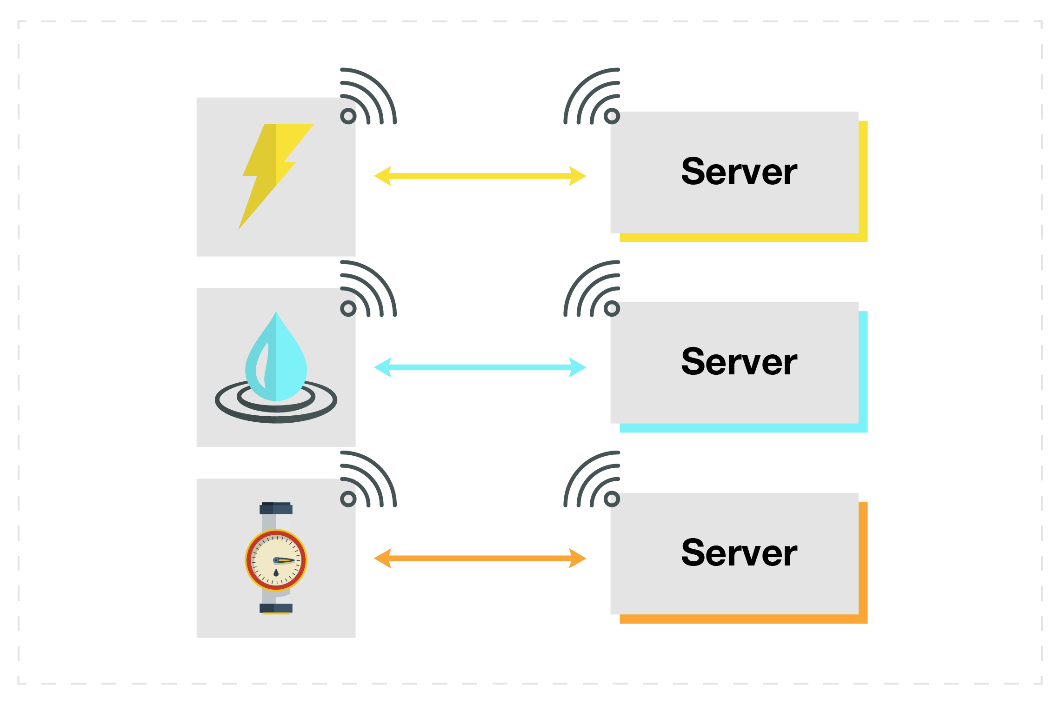
\includegraphics[width=8cm]{img/intro/esquema_comunicacion_old.png}
        \caption{\textbf{Esquema de comunicación de equipos de distintos fabricantes}}
        \textbf{\small Fuente: Elaboración propia}
        \label{fig:old_schema}
    \end{figure}
\end{itemize}

% Puntualizar o escribir como párrafo normal?
A raíz de estos factores considerados como problemática y además de los beneficios adicionales que se
tendría, se propone un prototipo que realice una lectura remota de los servicios básicos mediante el
reconocimiento de caracteres, es decir, un sistema de captura de imágenes de fácil y rápido montaje, 
que pueda implementarse a uno o mas medidores, que a través de un solo canal de comunicación, regulado bajo
normativa boliviana, envié dicha imagen (o imágenes) a un servidor donde, tras un procesamiento, se pueda 
almacenar el valor del consumo del servicio, como metadata, en una base de datos. Como se puede ver en \ref{fig:new_schema}
\begin{figure}[H]
    \centering
    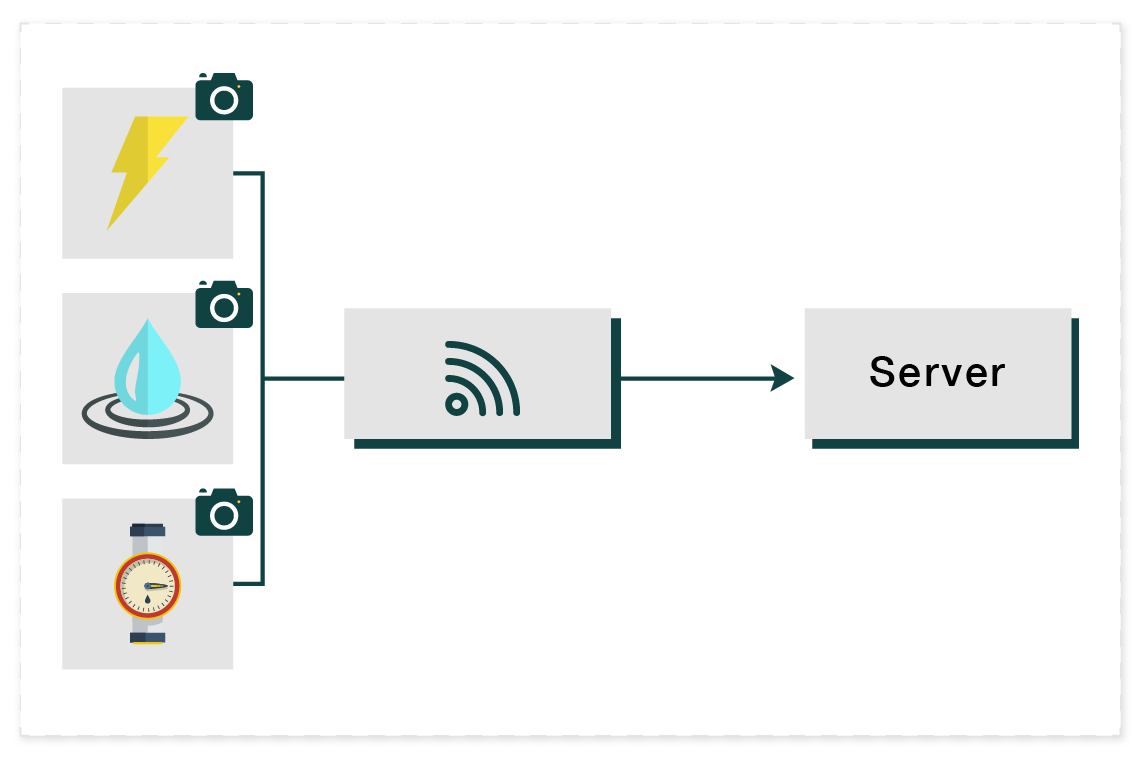
\includegraphics[width=8cm]{img/intro/esquema_comunicacion_new.png}
    \caption{\textbf{Esquema de comunicación propuesto}}
    \textbf{\small Fuente: Elaboración propia}
    \label{fig:new_schema}
\end{figure}



% Valdria la pena un gasto de mejora tecnologica sobre dispositivos antiguos? No tendriamos corte/activacion
% del servicio, pero por otro lado esta el despliegue rapido y que sea mas barato.

% Pros: Todavia tendriamos sistema antiguo como respaldo, despliegue rapido, adaptable, modular
% Cons: Un gasto que se realiza sobre tecnologia antigua (tanto en equipo como en instalacion),
        % centralizacion de datos? 

\section{Justificación}
La implementación de dicho sistema de lectura remota de servicios básicos conllevaría varios beneficios,
tanto es aspectos técnicos, económicos y sociales.

Técnicamente y como principal impacto estaría la centralización del envió de datos, el hecho de recolectar las
imágenes localmente y usar un solo canal de comunicación para el envió de estos archivos, nos permite implementar
una arquitectura mas simple, eliminando elementos innecesarios si hablamos de mediciones mixtas (de mas de un 
servicio). Ademas, en cualquier sistema electrónico sabemos que la mayor parte de la energía del dispositivo se
consume en la transmisión de datos, entonces centralizar el canal de comunicación también significa un ahorro
energético del sistema.

Se propone un sistema que este basado completamente en software libre, en cada nivel de implementación, por ende
los datos pueden entregarse a cualquier sistema tercero que cobranza o gestión y monitoreo. El acceso a esta información 
en casi tiempo real, llega a ser muy valiosa para cualquier tipo de servicio, si hablamos de consumo de luz, el SIN 
(Sistema interconectado nacional) puede realizar planificaciones de oferta o demanda futuras para la redistribución de 
energía o incluso para la compra/venta de esta. 
Si hablamos de fluidos, un gran beneficio seria la detección temprana de fugas, con una simple correlación de caudales
- la cantidad de fluido que sale del proveedor de servicio tiene que ser igual a las que llegan a las residencias-
podemos detectar en que puntos tenemos perdidas de manera mas rápida.
% Verificar si esto varia cuando el agua va a tanques

En cuanto al despliegue del sistema, debido a que el prototipo propuesto consistiría en un montaje simple de una cámara
para la captura de imagen de cada medidor, el sistema se puede instalar sin la necesidad de interrumpir el servicio al 
usuario y sin la necesidad de un plazo de testeo ya que todavía se tendría como respaldo el medidor antiguo, esto a 
diferencia de la instalación de un sistema de medición convencional donde se tendría que realizar un cambio de todo el
equipo de medición y pasar por un plazo de pruebas para ser instalado en toda una ciudad, ademas de la capacitación a
personal de la instalación de un dispositivo, siendo este escalable y modular para la cantidad de servicios necesarios.
% Considerar como se diferenciaria el firmware para cada tipo de medidor

En cuestiones económicas, debido a la topología del sistema, este seria mucho menos costoso que un sistema de medición
convencional, la eficiencia en su consumo energético implicarían costos menores en cuanto a la puesta en marcha del
sistema propuesto. Ademas de implícitamente generar ahorros en cuanto al uso de personal para la cobranza de los servicios
básicos y también ahorros en papel, debido a que no ya no sería necesario la impresión de boletas de cobranza e incluso
se podría sincronizar con un sistema de pagos en línea, como el que ya cuenta la empresa Elfec. El ultimo punto mencionado
podría también considerarse un beneficio ecológico.

Socialmente hablando, estamos atravesando una crisis mundial debido a la pandemia, donde la automatización de procesos
que desliga la intervención humana representa una mayor seguridad tanto para los empleados como para los consumidores del
servicio básico. Ademas que el sistema otorga la posibilidad de brindar la información de consumo al cliente en periodos
muchos mas cortos, para promover la concientización del uso de recursos no renovables, como el agua, o de los recursos
que generan huellas de carbono.

\section{Alcance y Delimitación}
El proyecto consiste en el desarrollo de un sistema de medición de servicios básicos
inteligente, aplicable a la normativa boliviana, mediante la captura de imagen del medidor,
el reconocimiento de los caracteres de la imagen, ademas del envió de esta a un servidor
para su procesamiento y obtención de la medida como dato. Se estudia el uso, manipulación y 
funcionamiento de medidores existentes en las residencias cochabambinas. Parte del proyecto 
también es el uso de componentes electrónicos, como la cámara, el controlador de esta y
el dispositivo que actuara como puerta de enlace de red. Se incurrió de igual manera en
la programación de la comunicación entre dispositivos finales, el código que recorta la
imagen, reconoce los números y los interpreta y asimismo de la configuración de una base 
de datos con la organización de los datos correspondientes. Se contempló el desarrollo de 
un sistema de fácil acople a cualquiera de los medidores analizados.\linebreak
Se contempló también la implementación de seguridad en la comunicación para evitar
'tampering' (termino usado para la manipulación ilegal de los consumos)

Por otro lado, debido a la comunicación inalámbrica entre los medidores de cada
servicio y el Gateway, hay una limitación en cuanto a la distancia que exista entre
estos y cualquier factor que pueda interferir con estas señales (como materiales que
realizan interferencia). Se tomó en cuenta la regulación de frecuencias establecidas
por ley en nuestro país, Bolivia.

Se limitó el desarrollo de componentes electrónicos para los dispositivos sensibles del
proyecto, es decir, dispositivos que requieran sistemas de transmisión inalámbrica sensibles
a interferencia, placas PCB de alta precisión o dispositivos que requieran de materiales
especiales con protecciones contra agua, gases u otros particulares.

La manipulación de esta información por las empresas prestadoras de servicio y la imposibilidad
de centralizar la información no es parte de este proyecto debido a que el carácter burocrático
esta fuera de las pertinencias del proyecto.
\chapter{Marco Teórico}
\section{IoT - Internet de las cosas}
	%Esta es mi teoría con esta cita \cite{WinNT}
	%Segunda cita \cite{WinNT1}
	%Tercera cita \cite{knuthwebsite}
	%Cuarta cita \cite{test}

\section{Medidores de servicios básicos}
    \subsection{Medidores mecánicos y electromecánicos}
    \subsection{Medidores electrónicos}
    \subsection{Medidores inteligentes}
\section{Microcontroladores}
    Este es un ejemplo de tablas
    \begin{table}[ht!]
		\begin{center}
				\begin{tabular}{l c c}
			1 & 2 & 3 \\ \hline
			4 & 5 & 6\\
			7&8&9\\
		\end{tabular}	
		\end{center}

		\caption{Tabla de ejemplo}
	\end{table}
\section{Cámaras}
\section{OCR - Reconocimiento óptico de caracteres}
\section{Bases de datos}	
\chapter{Desarrollo del proyecto}
\chapter{Resultados y validación}
\section{Análisis de costos}
\chapter{Conclusiones y Recomendaciones}
\section{Conclusiones}
\section{Recomendaciones}

\newpage
	\bibliography{biblio}
	\bibliographystyle{ieeetr}
	%\printbibliography
\appendix
\chapter{Anexos}
%\section*{Anexos}
%\addcontentsline{toc}{section}{Anexos}
%\appendix
%\begin{appendices}
%	\section{Lo demás}
%	\end{appendices}

\end{document}


